\graphicspath{{./Appendix/Figs/}}

\cleardoublepage

\chapter{Wind Tunnel Results}
\label{app:wtr}

\begin{figure}[H]
    \centering
    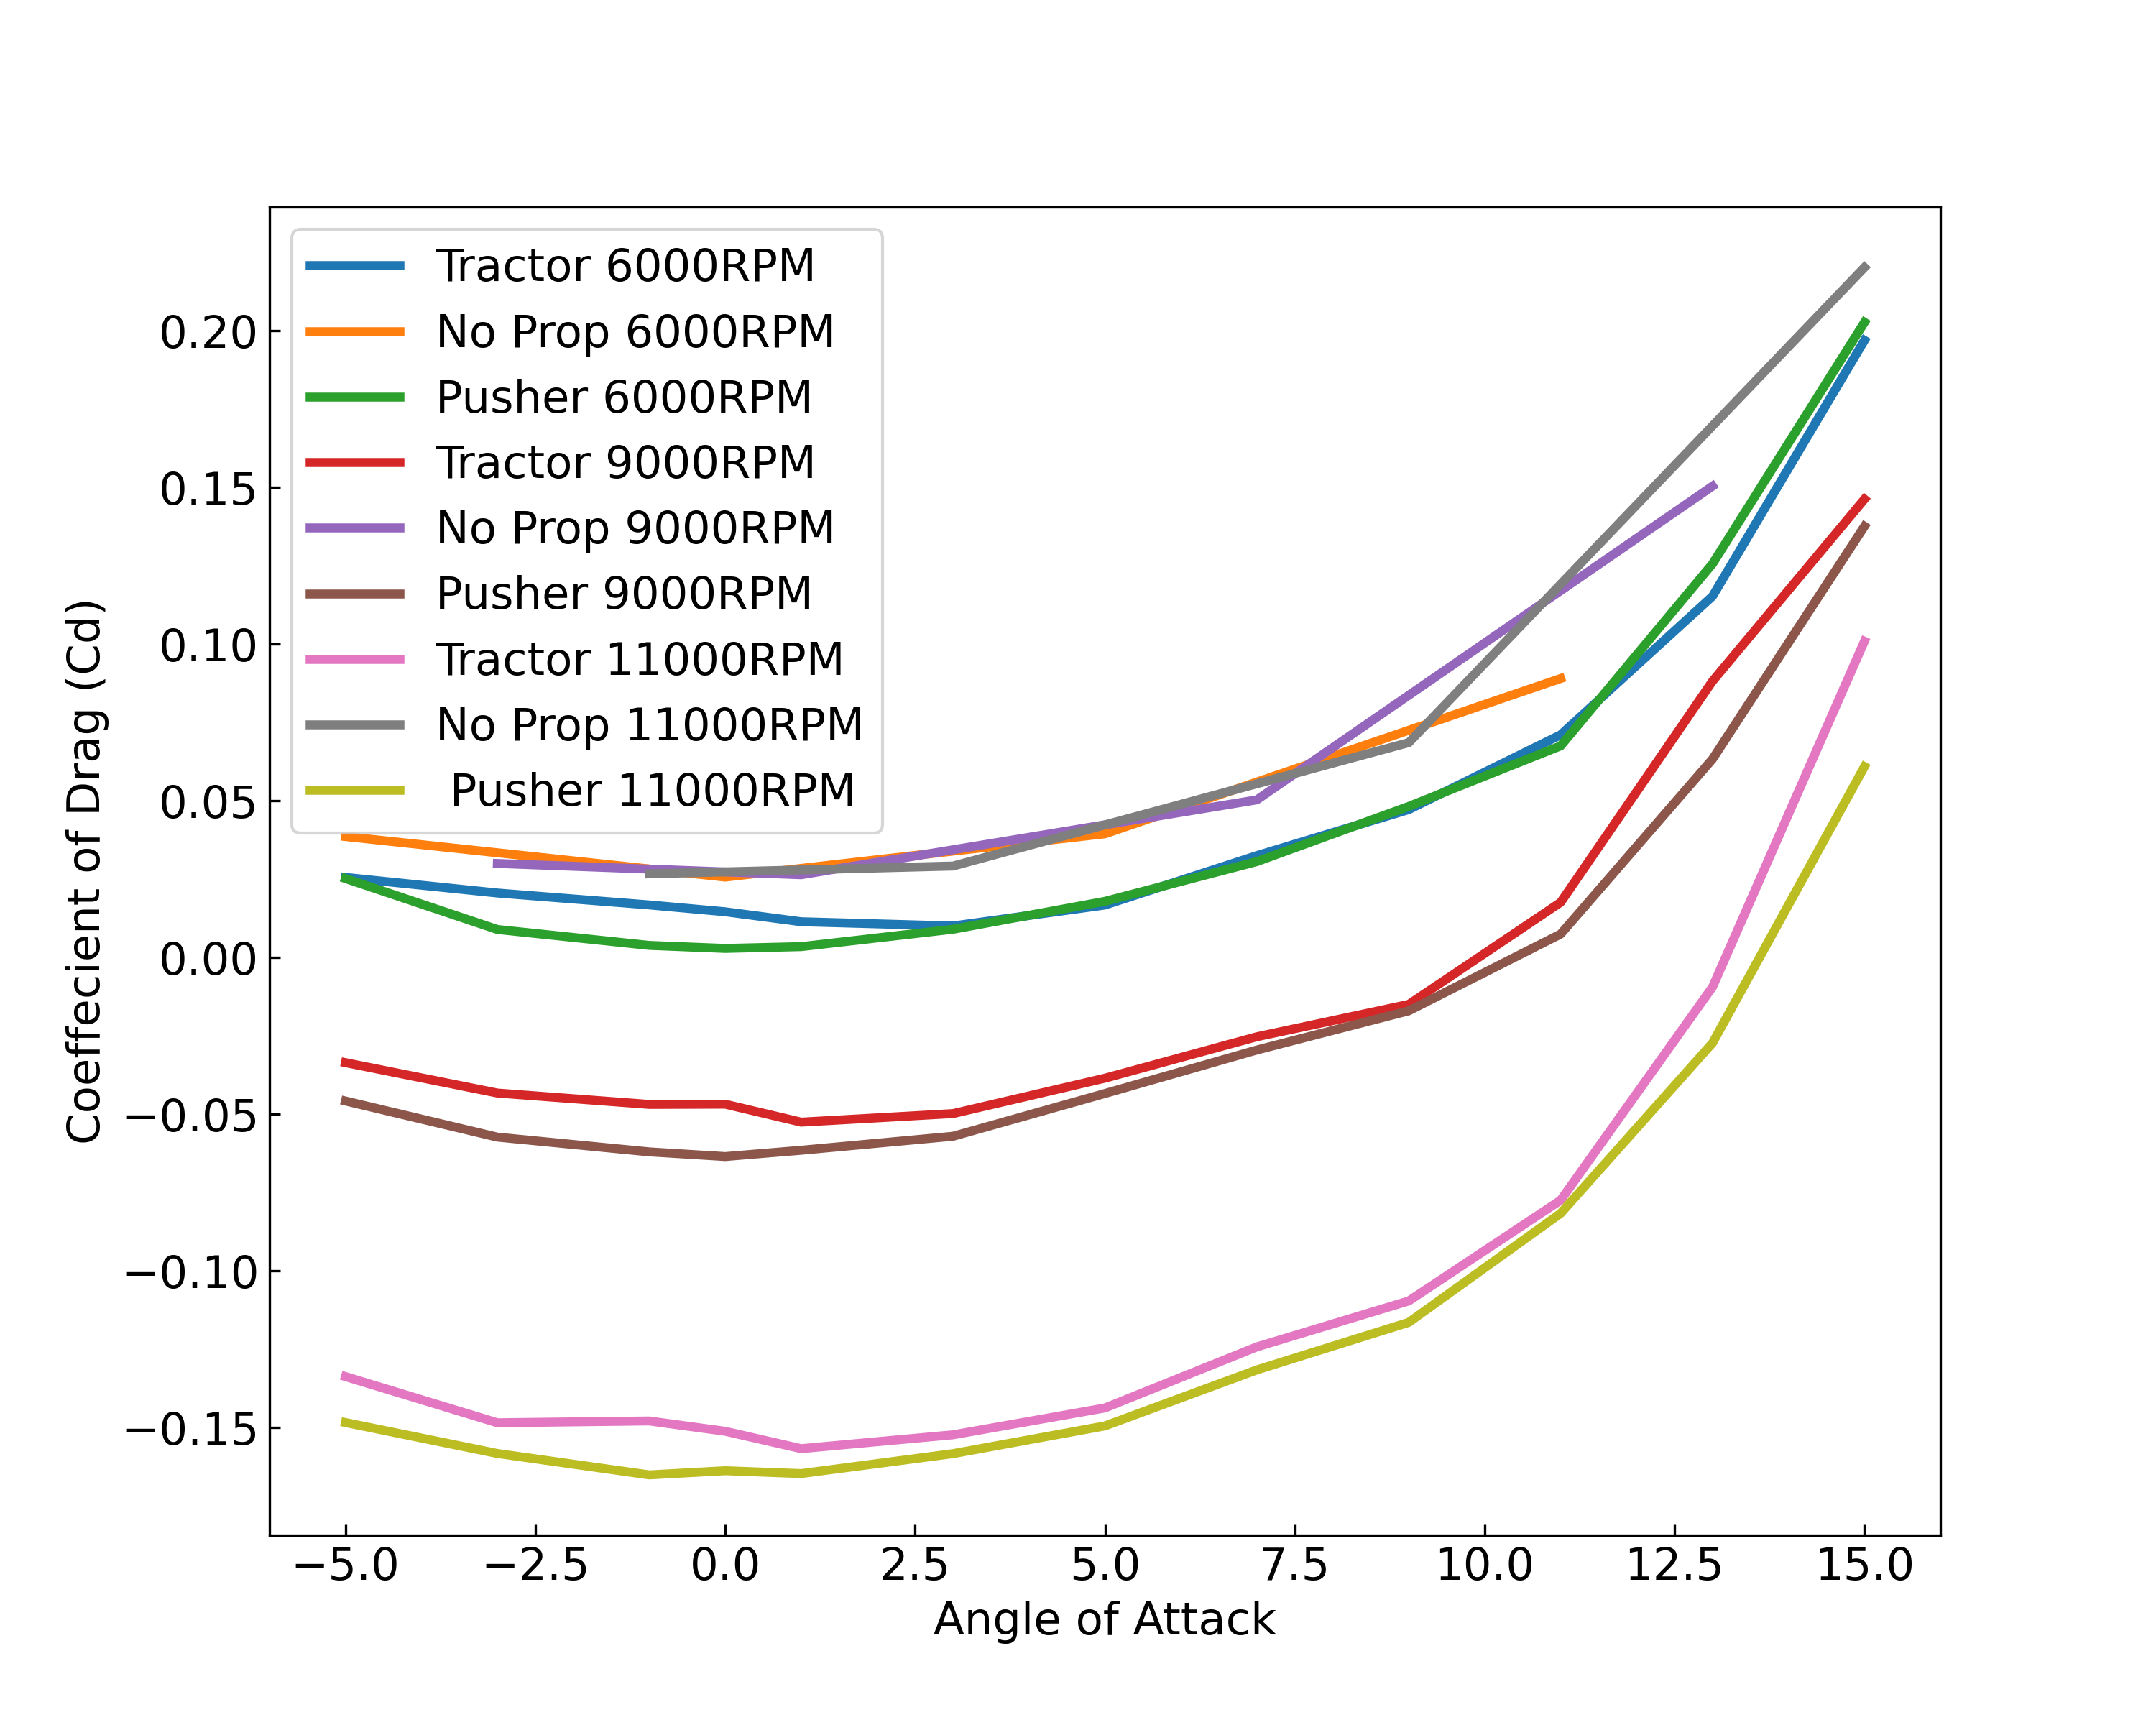
\includegraphics[scale = 0.7]{05_Results/Figs/Cd/10ms_Cd.png}
    \caption{Coefficient of drag variation at 20ms airspeed for the tractor, pusher and no propeller configuration}
    \label{fig:Cd_20ms}
\end{figure}

% \chapter{Work Health and Safety}
% \label{app:whs}

% Ensuring that a safe work environment is present for everyone is critical to reducing injury and illness and increases productivity. In order to do this it is a requirement of the Australian Work, Health and Safety laws to do the following\cite{}: \todo{cite}
% % https://business.gov.au/risk-management/health-and-safety/work-health-and-safety

% \begin{itemize}
%     \item Provide a safe work environment
%     \item Provide and maintain safe machinery and structures
%     \item Provide safe ways of working
%     \item Ensure safe use, handling and storage of machinery, structures and substances
%     \item Provide and maintain adequate facilities
%     \item Provide any information, training, instruction or supervision needed for safety
%     \item Monitor the health of workers and conditions at the workplace.
% \end{itemize}

% Workers also have several obligations to both themselves and those around them. They must\cite{}:

% \begin{itemize}
%     \item Take care of their own health and safety
%     \item Take care not to do anything that could hurt others
%     \item Follow WHS instructions
%     \item Follow the workplace’s WHS policies and procedures
% \end{itemize}

% This section analyses the significant health and safety concerns in regards to the development, collation of data and writing of this thesis. The main topics covered are physical health, mental health and wind tunnel safety.




% \todo{change this to a cite}
% \begin{figure}[H]
%   \centering
%   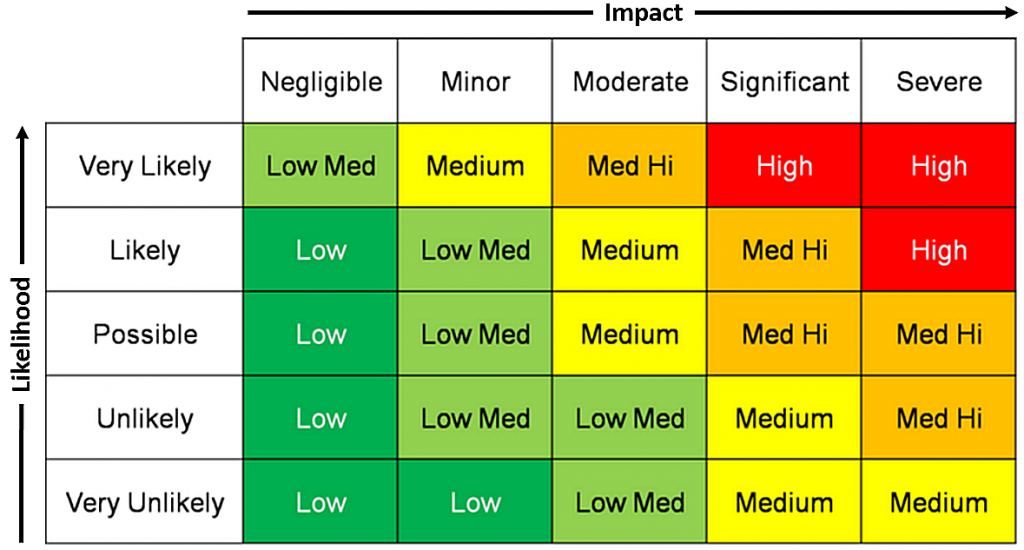
\includegraphics[width=\textwidth]{risk_matrix.png}
%   \caption[Risk matrix.]{Risk matrix. From \url{https://www.armsreliability.com/page/resources/blog/beyond-the-risk-matrix}.}
%   \label{fig:risk_matrix}
% \end{figure}




% \section{Physical Health}
% This thesis involved long hours of repetitive desk tasks. These tasks done over long durations led to bad posture, wrist strain, eye strain



% In a standard office, work is often long, repetitive, and stationary. Bad posture, uncomfortable chairs, mispositioned monitors, wrist strain over cramped keyboards, poor lighting or glare are just a few of the most common risks and hazards to physical health. 

% At Accenture and home, the following precautions were observed:
% \begin{enumerate}
%   \item Education on the proper position to work in was studied from \ref{fig:posture_desk}. Notably, the height of the chair is set to the appropriate height to allow feet to rest in an almost \SI{90}{\deg} angle, the top of the monitor edge at eye level, and the monitor slightly tilted up to equalise the distance to all corners of the screen. 
%   \item Good chairs were selected. I purchased a Herman Miller Aeron chair for work at home, known for its world-renowned ergonomics. 
%   \item Used a second external monitor to relieve neck strain, as it is possible to adjust the monitor's position to the optimal position. This also provided a significant productivity boost. The brightness was also adequately adjusted to bring the most comfort to the eyes. 
%   \item A standing desk was purchased for working at home. 
%   \item Regular breaks were taken with the team during the time at the office. 
%   \item An ergonomic keyboard, the Kinesis Advantage 2, was used to relieve wrist strain and improve productivity with the features such as macros. 
% \end{enumerate}

% \begin{figure}[H]
%   \centering
%   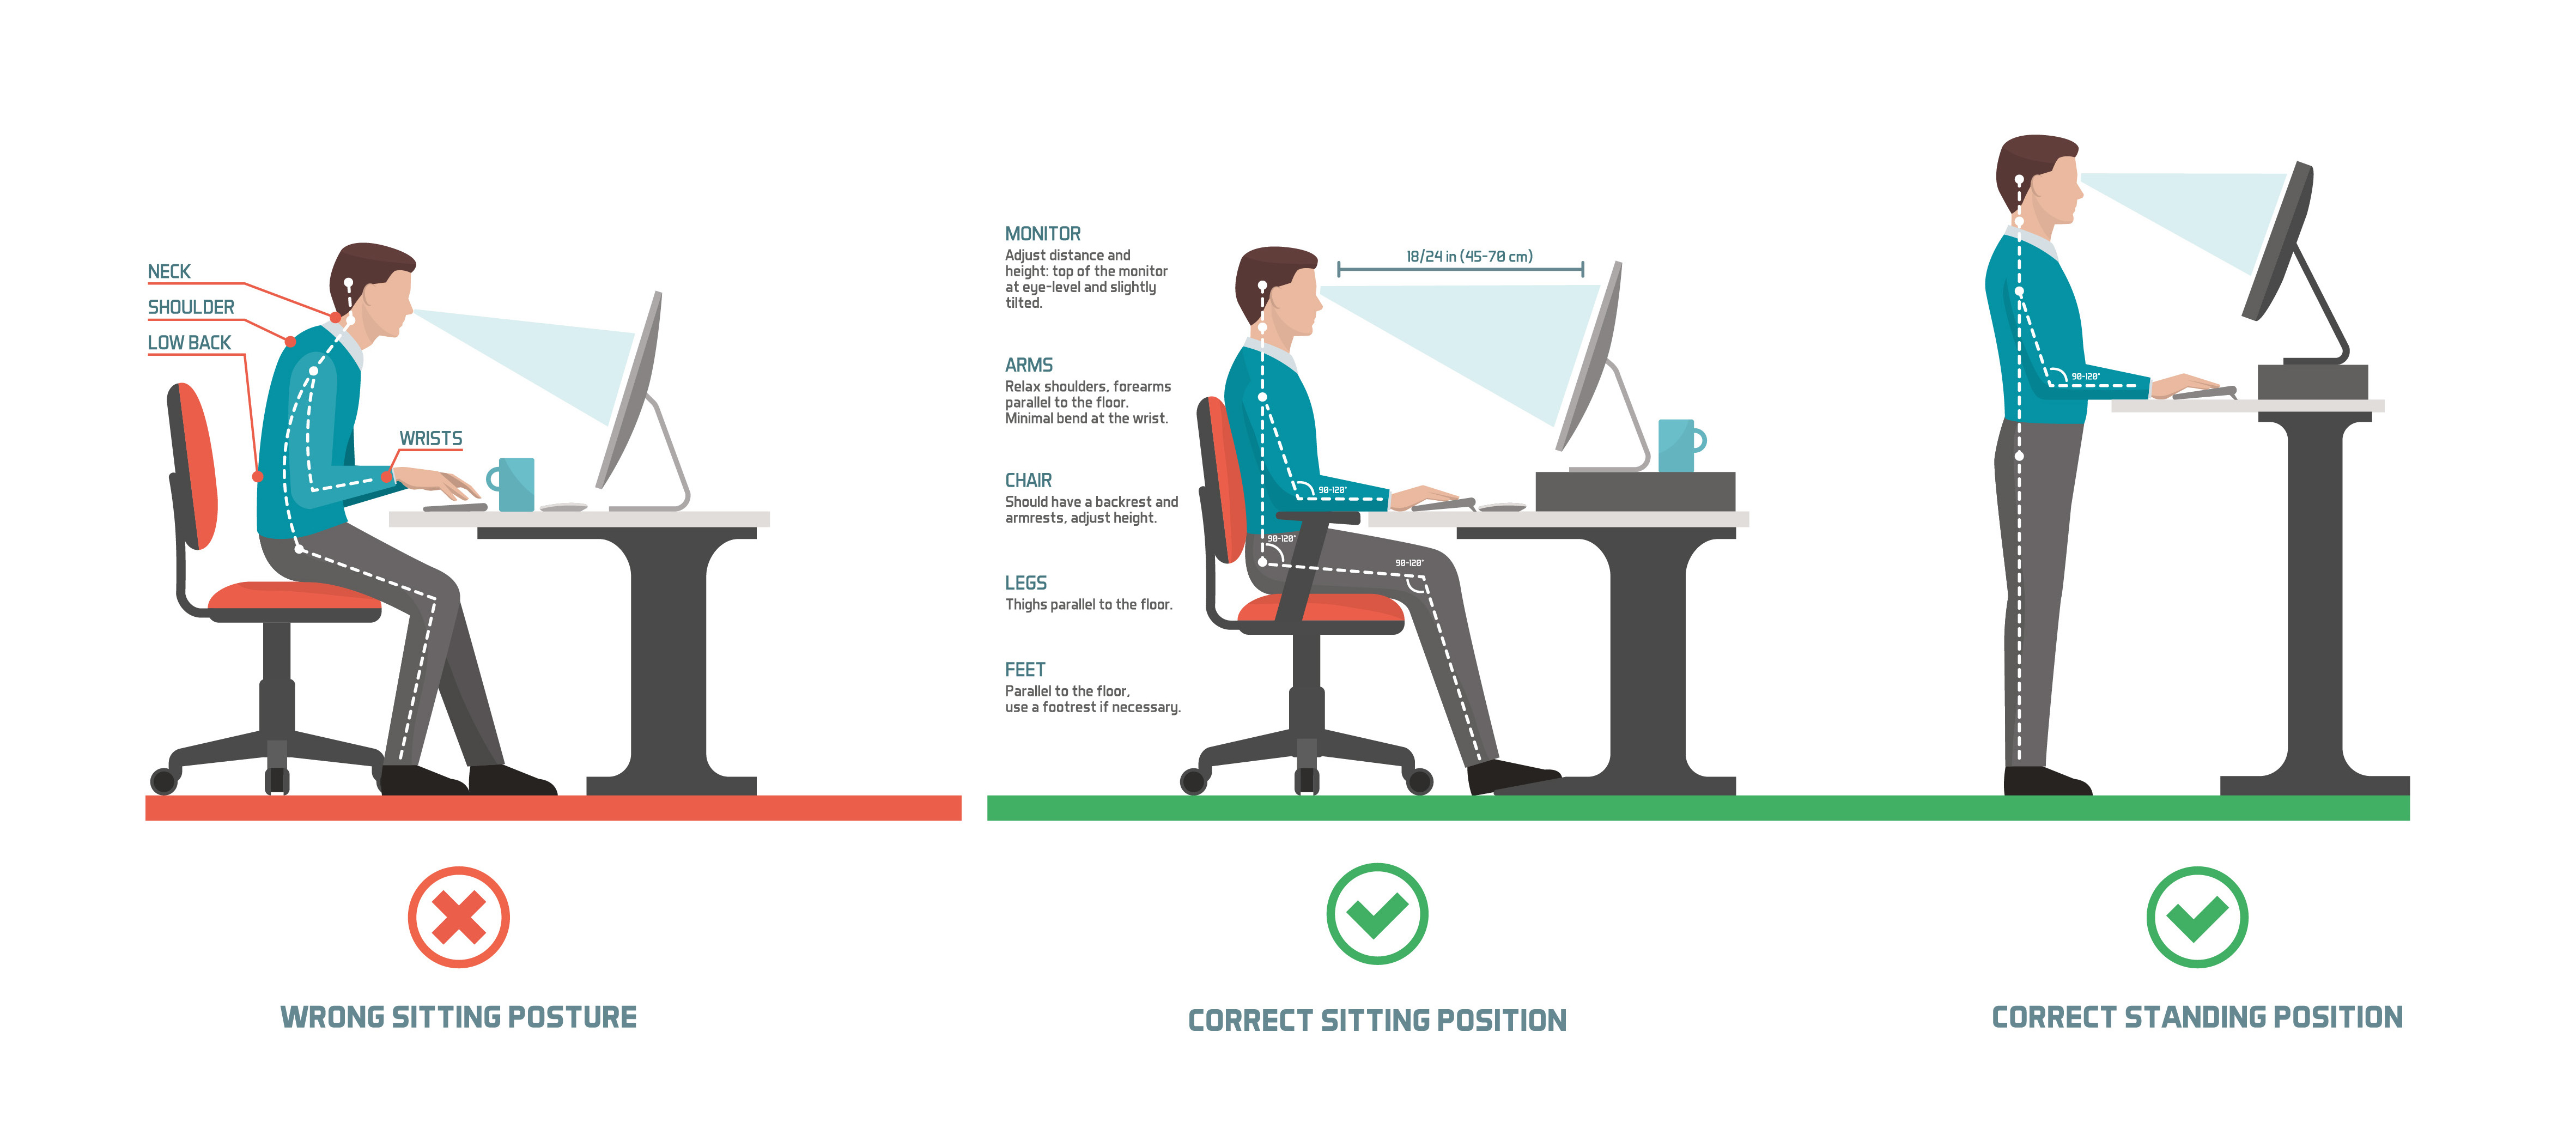
\includegraphics[width=\textwidth]{posture_desk.jpeg}
%   \caption[Best posture at a desk.]{Best posture at a desk. From: \url{https://healthandbalance.com.au/workstation-desk-posture-ergonomics/}}
%   \label{fig:posture_desk}
% \end{figure}

% Although there are many sources of long-term physical issues, these can be easily managed with awareness and mitigated effectively, resulting in a low level of risk. 

% \section{Covid-19 precautions}
% Covid-19 has undeniably impacted the world in many ways. This highly infectious disease caused major lockdowns and shifted work from the office to the home for extended periods. In order to follow national and state requirements, Accenture and employees worked remotely and suspended office visits. Return to the office was first announced in mid-November, where a number of precautions were followed:

% \begin{enumerate}
%   \item All state and national requirements were followed, including masks in public indoor areas and on transport, QR code check-ins in all locations required, and mandatory bookings for visits to the office.
%   \item Social distancing in all public areas. 
%   \item Sanitising hands on every entry to the office.
%   \item Disallowing guest visits to the office. 
% \end{enumerate}

% Although the severity of symptoms one suffers from contracting Covid-19 vary wildly in the younger age group, the potential to be sick for a week or more, in addition to the mandatory self-isolation period, is highly disruptive to work and the greater population. As such, the threat of Covid-19 results in high risk. 


% \section{Mental health}
% Mental health is an often under-looked part of one's health. It varies greatly from person to person, and many factors play into one's overall mental health, including social health, work-life balance, and financial status. Without careful consideration, planning and awareness of one's mental health, the employee's productivity may drop sharply. 

% A number of precautions were taken to care for my mental health:
% \begin{enumerate}
%   \item Ensuring I was enjoying the work I was doing. I transferred internally between teams to find more exciting work that I could grow and learn in while also finding a more relevant thesis topic aligned with my interests. 
%   \item Coming into the office when practical. Although there were many days where I was the only team member in the office, being able to experience the office, grab hot drinks in the morning with colleagues, and work in an environment separate from home was very beneficial.
%   \item Preventing work hours from extending into my personal time too often. 
% \end{enumerate}

% Mental health is a complex risk to quantify since it is difficult to measure and includes many factors. Overall the onus is mainly on the employee to ensure they take the proper precautions and use the available resources such as sick leave or personal time off. Particularly with the challenging program that is ESIPS, this risk is categorised as a moderate risk. 
